
\subsubsection{Analisi Derivazioni e Ridondanze}
In questa prima fase analizziamo le ridondanze già presenti. L' unica riscontrata riguarda l'attributo importo ridondante per le entità Contratto di Assistenza on Center e Fattura legate dalla relazione Esecuzione Contratto (operazioni 6, 10, 24, 30, 39), dove l'importo è presente in entrambe le entità.
L'attributo importo nell'entità Fattura è vincolato dalla decisione di non conservare tutti i cataloghi dei fornitori per questioni di spazio. Quindi aggiornando mensilmente i prezzi dei cataloghi si perde la possibilità di andare a cercare il valore di un prodotto in un certo arco temporale se non quello attuale, e questo renderebbe impossibile calcolare l'importo di una fattura a posteriori. Per questo motivo l'attributo importo deve essere presente e lo si considera ridondante nell'entità del contratto di assistenza on center piuttosto che nella fattura.
\newline\newline
\centerline{\textbf{ATTRIBUTO IMPORTO IN CONTRATTO DI ASSISTENZA ON CENTER}}
\newline
\centerline{\textbf{CON RIDONDANZA}}
\begin{table}[H]
\centering
\caption{Operazione 6}
\begin{tabular}{llll}
\\ \hline
\multicolumn{1}{|l|}{\textbf{CONCETTO}} & \multicolumn{1}{l|}{\textbf{COSTRUTTO}} & \multicolumn{1}{l|}{\textbf{ACCESSI}} & \multicolumn{1}{l|}{\textbf{TIPO}} \\ \hline
\multicolumn{1}{|l|}{FATTURA}
& \multicolumn{1}{l|}{E}                  & \multicolumn{1}{l|}{1}                & \multicolumn{1}{l|}{S}             \\ \hline
\end{tabular}
\end{table}


\begin{table}[H]
\centering
\caption{Operazione 10}
\begin{tabular}{llll}
\\ \hline
\multicolumn{1}{|l|}{\textbf{CONCETTO}} & \multicolumn{1}{l|}{\textbf{COSTRUTTO}} & \multicolumn{1}{l|}{\textbf{ACCESSI}} & \multicolumn{1}{l|}{\textbf{TIPO}} \\ \hline
\multicolumn{1}{|l|}{Contratto di assistenza on center}
& \multicolumn{1}{l|}{E}                  & \multicolumn{1}{l|}{1}                & \multicolumn{1}{l|}{L}             \\ \hline
\multicolumn{1}{|l|}{Fattura}             & \multicolumn{1}{l|}{E}                  & \multicolumn{1}{l|}{1}                & \multicolumn{1}{l|}{L}             \\ \hline
\multicolumn{1}{|l|}{Esecuzione Contratto}     & \multicolumn{1}{l|}{R}                  & \multicolumn{1}{l|}{2}                & \multicolumn{1}{l|}{S}             \\ \hline
\multicolumn{1}{|l|}{Esecuzione Contratto}
& \multicolumn{1}{l|}{R}                  & \multicolumn{1}{l|}{2}                & \multicolumn{1}{l|}{L}             \\ \hline
\end{tabular}
\end{table}

\begin{table}[H]
\centering
\caption{Operazione 24}
\begin{tabular}{llll}
\\ \hline
\multicolumn{1}{|l|}{\textbf{CONCETTO}} & \multicolumn{1}{l|}{\textbf{COSTRUTTO}} & \multicolumn{1}{l|}{\textbf{ACCESSI}} & \multicolumn{1}{l|}{\textbf{TIPO}} \\ \hline
\multicolumn{1}{|l|}{Esecuzione Contratto}
& \multicolumn{1}{l|}{R}                  & \multicolumn{1}{l|}{1}                & \multicolumn{1}{l|}{L}             \\ \hline
\end{tabular}
\end{table}

\begin{table}[H]
\centering
\caption{Operazione 25}
\begin{tabular}{llll}
\\ \hline
\multicolumn{1}{|l|}{\textbf{CONCETTO}} & \multicolumn{1}{l|}{\textbf{COSTRUTTO}} & \multicolumn{1}{l|}{\textbf{ACCESSI}} & \multicolumn{1}{l|}{\textbf{TIPO}} \\ \hline
\multicolumn{1}{|l|}{Esecuzione Contratto}
& \multicolumn{1}{l|}{R}                  & \multicolumn{1}{l|}{1*1=1}                & \multicolumn{1}{l|}{L}             \\ \hline
\end{tabular}
\end{table}

\begin{table}[H]
\centering
\caption{Operazione 30}
\begin{tabular}{llll}
\\ \hline
\multicolumn{1}{|l|}{\textbf{CONCETTO}} & \multicolumn{1}{l|}{\textbf{COSTRUTTO}} & \multicolumn{1}{l|}{\textbf{ACCESSI}} & \multicolumn{1}{l|}{\textbf{TIPO}} \\ \hline
\multicolumn{1}{|l|}{Fattura}
& \multicolumn{1}{l|}{E}                  & \multicolumn{1}{l|}{1}                & \multicolumn{1}{l|}{L}             \\ \hline
\end{tabular}
\end{table}

\begin{table}[H]
\centering
\caption{Operazione 39}
\begin{tabular}{llll}
\\ \hline
\multicolumn{1}{|l|}{\textbf{CONCETTO}} & \multicolumn{1}{l|}{\textbf{COSTRUTTO}} & \multicolumn{1}{l|}{\textbf{ACCESSI}} & \multicolumn{1}{l|}{\textbf{TIPO}} \\ \hline
\multicolumn{1}{|l|}{Fattura}
& \multicolumn{1}{l|}{R}                  & \multicolumn{1}{l|}{1*12=12}                & \multicolumn{1}{l|}{L}             \\ \hline
\end{tabular}
\end{table}


\newline\newline\centerline{\textbf{SENZA RIDONDANZA}}
\begin{table}[H]
\centering
\caption{Operazione 6}
\begin{tabular}{llll}
\\ \hline
\multicolumn{1}{|l|}{\textbf{CONCETTO}} & \multicolumn{1}{l|}{\textbf{COSTRUTTO}} & \multicolumn{1}{l|}{\textbf{ACCESSI}} & \multicolumn{1}{l|}{\textbf{TIPO}} \\ \hline
\multicolumn{1}{|l|}{FATTURA}
& \multicolumn{1}{l|}{E}                  & \multicolumn{1}{l|}{1}                & \multicolumn{1}{l|}{S}             \\ \hline
\end{tabular}
\end{table}


\begin{table}[H]
\centering
\caption{Operazione 10}
\begin{tabular}{llll}
\\ \hline
\multicolumn{1}{|l|}{\textbf{CONCETTO}} & \multicolumn{1}{l|}{\textbf{COSTRUTTO}} & \multicolumn{1}{l|}{\textbf{ACCESSI}} & \multicolumn{1}{l|}{\textbf{TIPO}} \\ \hline
\multicolumn{1}{|l|}{Fattura}             & \multicolumn{1}{l|}{E}                  & \multicolumn{1}{l|}{1}                & \multicolumn{1}{l|}{L}             \\ \hline
\multicolumn{1}{|l|}{Esecuzione Contratto}     & \multicolumn{1}{l|}{R}                  & \multicolumn{1}{l|}{1}                & \multicolumn{1}{l|}{S}             \\ \hline
\multicolumn{1}{|l|}{Esecuzione Contratto}
& \multicolumn{1}{l|}{R}                  & \multicolumn{1}{l|}{1}                & \multicolumn{1}{l|}{L}             \\ \hline
\end{tabular}
\end{table}

\begin{table}[H]
\centering
\caption{Operazione 24}
\begin{tabular}{llll}
\\ \hline
\multicolumn{1}{|l|}{\textbf{CONCETTO}} & \multicolumn{1}{l|}{\textbf{COSTRUTTO}} & \multicolumn{1}{l|}{\textbf{ACCESSI}} & \multicolumn{1}{l|}{\textbf{TIPO}} \\ \hline
\multicolumn{1}{|l|}{Esecuzione Contratto}
& \multicolumn{1}{l|}{R}                  & \multicolumn{1}{l|}{1}                & \multicolumn{1}{l|}{L}             \\ \hline
\multicolumn{1}{|l|}{Fattura}             & \multicolumn{1}{l|}{E}                  & \multicolumn{1}{l|}{1}                & \multicolumn{1}{l|}{L}             \\ \hline
\end{tabular}
\end{table}

\begin{table}[H]
\centering
\caption{Operazione 25}
\begin{tabular}{llll}
\\ \hline
\multicolumn{1}{|l|}{\textbf{CONCETTO}} & \multicolumn{1}{l|}{\textbf{COSTRUTTO}} & \multicolumn{1}{l|}{\textbf{ACCESSI}} & \multicolumn{1}{l|}{\textbf{TIPO}} \\ \hline
\multicolumn{1}{|l|}{Esecuzione Contratto}
& \multicolumn{1}{l|}{R}                  & \multicolumn{1}{l|}{1*1=1}                & \multicolumn{1}{l|}{L}             \\ \hline
\multicolumn{1}{|l|}{Fattura}             & \multicolumn{1}{l|}{E}                  & \multicolumn{1}{l|}{1*1=1}                & \multicolumn{1}{l|}{L}             \\ \hline
\end{tabular}
\end{table}

\begin{table}[H]
\centering
\caption{Operazione 30}
\begin{tabular}{llll}
\\ \hline
\multicolumn{1}{|l|}{\textbf{CONCETTO}} & \multicolumn{1}{l|}{\textbf{COSTRUTTO}} & \multicolumn{1}{l|}{\textbf{ACCESSI}} & \multicolumn{1}{l|}{\textbf{TIPO}} \\ \hline
\multicolumn{1}{|l|}{Fattura}
& \multicolumn{1}{l|}{E}                  & \multicolumn{1}{l|}{1}                & \multicolumn{1}{l|}{L}             \\ \hline
\end{tabular}
\end{table}

\begin{table}[H]
\centering
\caption{Operazione 39}
\begin{tabular}{llll}
\\ \hline
\multicolumn{1}{|l|}{\textbf{CONCETTO}} & \multicolumn{1}{l|}{\textbf{COSTRUTTO}} & \multicolumn{1}{l|}{\textbf{ACCESSI}} & \multicolumn{1}{l|}{\textbf{TIPO}} \\ \hline
\multicolumn{1}{|l|}{Fattura}
& \multicolumn{1}{l|}{R}                  & \multicolumn{1}{l|}{1*12=12}                & \multicolumn{1}{l|}{L}             \\ \hline
\end{tabular}
\end{table}


\begin{table}[H]
\centering
\caption{Costo Operazioni con ridondanza}
\label{my-label}
\resizebox{\textwidth}{!}{%
\begin{tabular}{|l|l|l|l|}
\hline
\textbf{OPERAZIONE}               & \textbf{COSTO} & \textbf{FREQUENZA} & \textbf{TOTALE} \\ \hline
6                                & 1             & 90             & 90
\\ \hline
10                                & 6              & 1              & 6
\\ \hline
24                                & 1              & 8             & 8
\\ \hline
25                                & 1              & 2              & 2
\\ \hline
30                                & 1              & 30             & 30
\\ \hline
39                                & 12             & 1             & 12
\\ \hline
COSTO OPERAZIONI CON RIDONDANZA & 22        &                    &   \hl{148}             \\ \hline
\end{tabular}
}
\end{table}


\begin{table}[H]
\centering
\caption{Costo Operazioni senza Ridondanza}
\label{my-label}
\resizebox{\textwidth}{!}{%
\begin{tabular}{|l|l|l|l|}
\hline
\textbf{OPERAZIONE}             & \textbf{COSTO} & \textbf{FREQUENZA} & \textbf{TOTALE} \\ \hline
6                                & 1             & 90             & 90
\\ \hline
10                                & 3              & 1              & 3
\\ \hline
24                                & 2              & 8             & 16
\\ \hline
25                                & 2              & 2              & 4
\\ \hline
30                                & 1              & 30             & 30          \\ \hline
39                                & 12             & 1             & 12
\\ \hline
COSTO OPERAZIONI SENZA RIDONDANZA & 21        &                    &  \hl{155}               \\ \hline
\end{tabular}
}
\end{table}

\newline
Dai calcoli effettuati risulta evidente una differenza davvero minima per quanto concerne il costo delle operazioni. In questo caso si sceglie di non rindondare l'attributo, per avere un guadagno di memoria, al prezzo di qualche operazioni in più.
\newline
Inoltre dall'analisi del modello non è stata riscontrata la possibilità di inserire ulteriori attributi ridondanti.


\newpage
\subsubsection{Eliminazione Delle Gerarchie}

Nel nostro schema concettuale sono presenti 5 generalizzazioni. Le Entità coinvolte sono "PA, Azienda o Persona", "Cliente", "Richiesta sul Mepa", "Prodotto o servizio", "Prodotto".
\newline
Abbiamo deciso di procedere nel seguente modo:

\paragraph{PA, Azienda o Persona}
Per quanto riguarda l'entità PA, Azienda o Persona, abbiamo scelto di accorpare il genitore della generalizzazione nelle entità figlie. Questo perchè i clienti e i fornitori hanno rapporti con l'azienda piuttosto diversi tra loro, quindi la separazione comporta una suddivisione concettuale che migliora la chiarezza dello schema.
\paragraph{Cliente}
Per l'entità Cliente si è optato di mantenere il genitore e mantenere le entità figlie, in quanto un eventuale accorpamento del genitore nelle entità figlie complicherebbe lo schema, viste le numerose relazioni che ha il genitore. Abbiamo sostituito la generalizzazione con delle relazioni, denominate "Specificazione Privato" e "Specificazione PA".
\paragraph{Richiesta sul Mepa}
In merito all'entità Richiesta sul Mepa, si è scelto l'accorpamento del genitore della generalizzazione nelle entità figlie. Si avrebbe potuto accorpare le entità figlie nel genitore, utilizzando degli attributi che possono assumere il valore NULL per poter distinguire appunto le due entità, ma ci sembra più opportuno mantenere distinte le entità Gara pubblica e Trattativa diretta in quanto esse sono, nella realtà pratica, due concetti logicamente separati. Il mantenimento della loro suddivisione permette quindi una maggior comprensibilità dello schema.
\paragraph{Prodotto o Servizio}
Per quanto riguarda l'entità Prodotto o Servizio, abbiamo deciso di mantenere le entità figlie ed eliminare il genitore, in quanto ogni operazione che coinvolge il padre comprende almeno uno dei figli.
\paragraph{Prodotto}
Per l'entità Prodotto si è scelto di mantenere sia il padre che le entità figlie, dato che queste ultime hanno tanti attributi diversi, e l'accorpamento nell'entità genitore significherebbe avere tanti valori con valore NULL. Inoltre, un eventuale accorpamento del genitore nelle entità figlie risulterebbe piuttosto complicato, date le numerose relazioni che ha il padre e visto che le entità figlie sono molteplici.
Quindi, si è scelto di sostituire la generalizzazione con delle relazioni, una per ogni entità figlia. Le nuove relazioni sono denominate "Specificazione" più il nome dell'entità a cui si riferiscono.
\newline\newline
In seguito all'eliminazione delle generalizzazioni di Cliente e Prodotto, è necessario imporre delle nuove regole di vincolo, per evitare errori logici:

\begin{itemize}
  \item Ogni occorrenza di "Cliente" deve essere occorrenza o di "Privato" o di "Pubblica Amministrazione". Non potrà essere occorrenza contemporaneamente di entrambe queste entità.
  \item Ogni occorrenza di "Prodotto" deve essere occorrenza o di "Notebook" o di "Pc Desktop" o di "Monitor" o di "Stampante". Non potrà essere occorrenza contemporaneamente di due o più di queste entità.
\end{itemize}
\noindent
\textit{(Facciamo notare che, per non appesantire ulteriormente lo schema, abbiamo scelto di togliere alcuni prodotti e di mantenere solo "Notebook", "Pc Desktop", "Monitor", "Stampante".)}



\newpage
\begin{landscape} %inizia un foglio landscape

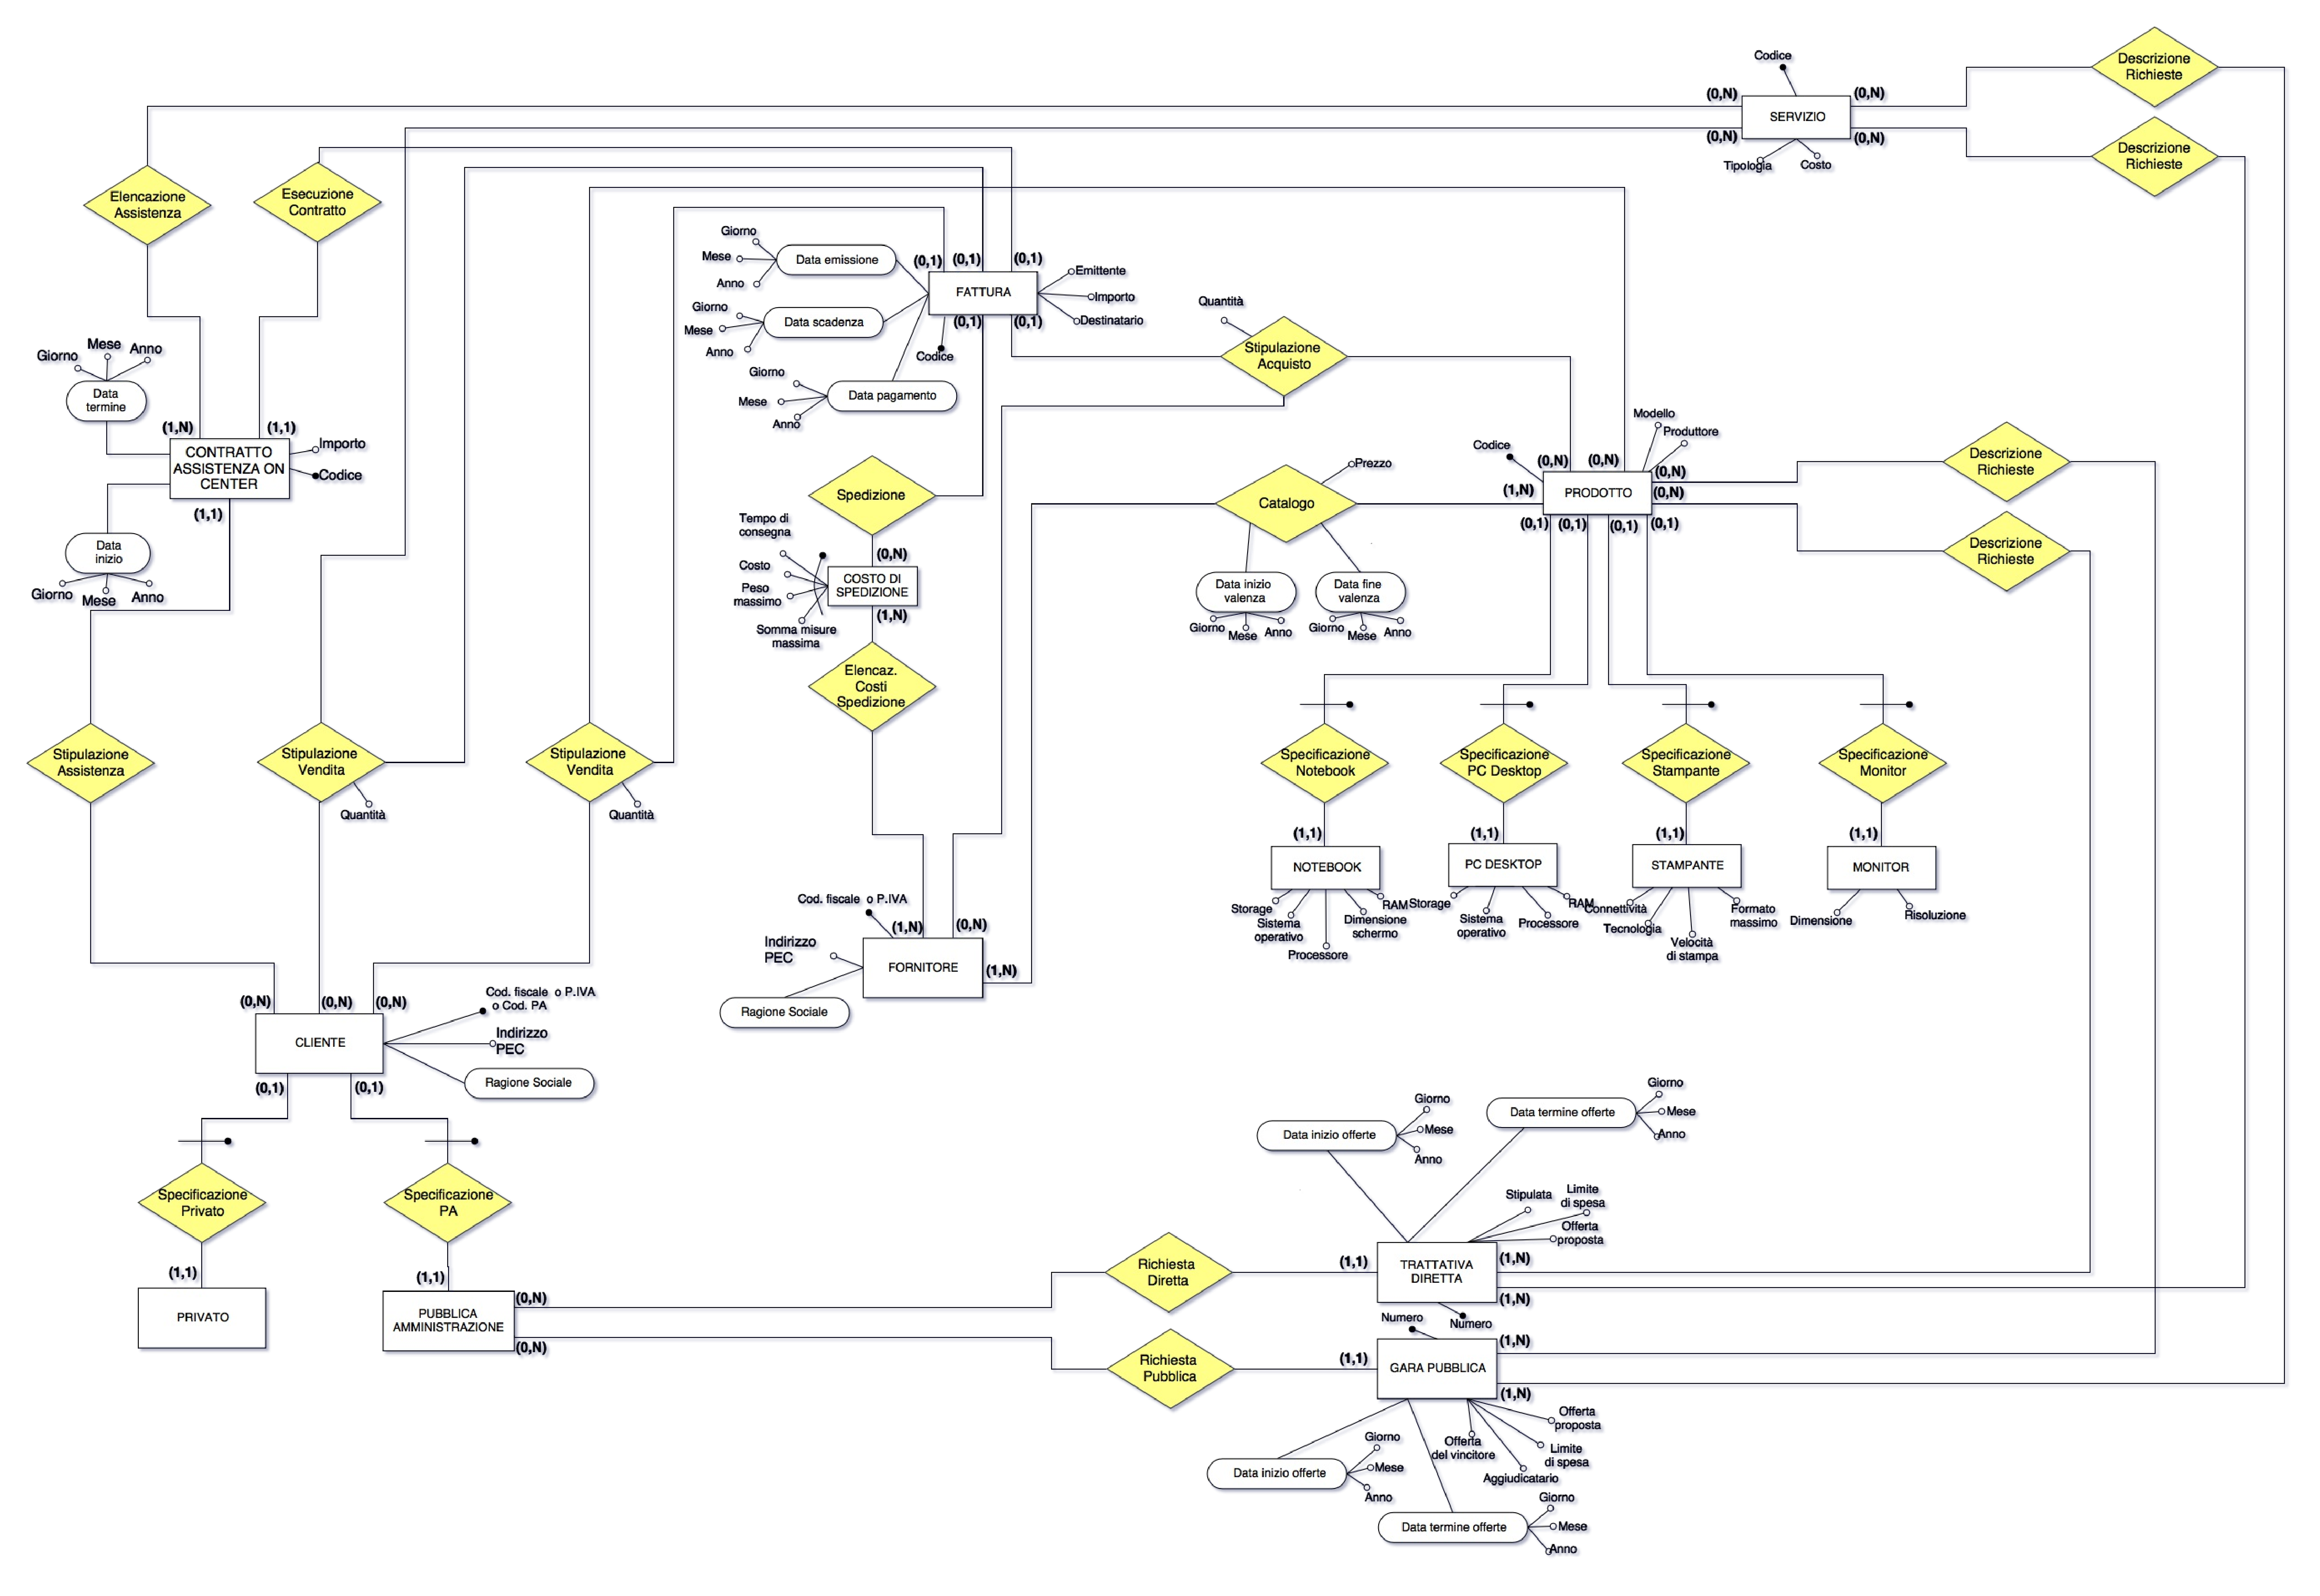
\includepdf[angle=90]{./immagini/modello_er_v3.pdf}

\end{landscape}


\newpage
\subsubsection{Eliminazione degli Attributi Multivalore}

Abbiamo individuato un solo attributo multivalore, l'attributo Telefono nelle entità Privato, Pubblica Amministrazione e Fornitore, in quanto abbiamo ritenuto che sia possibile che una di queste entità abbia più numeri di telefono associati.
\newline
Relativamente alle relazioni qui sopra citate abbiamo eseguito la ristrutturazione seguente:
\newline\newline

\noindent\makebox[\textwidth]{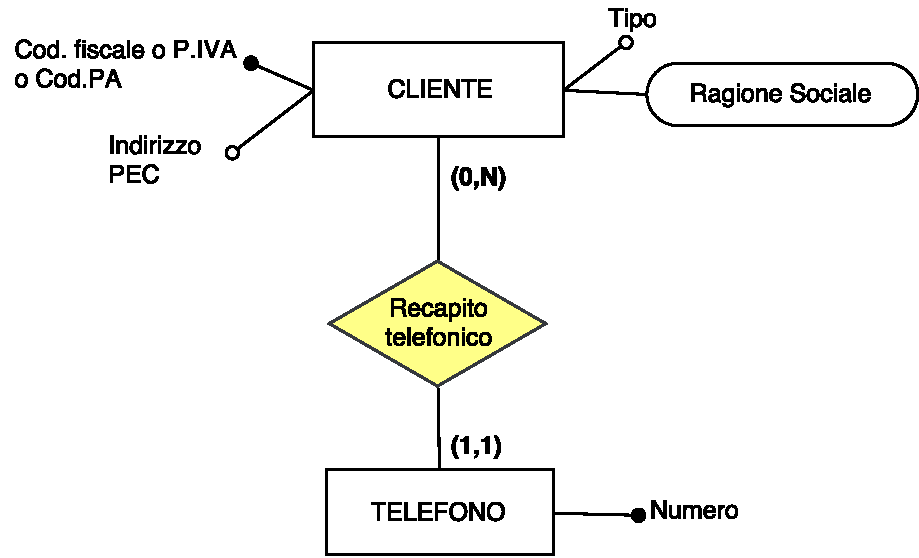
\includegraphics[width=0.7\linewidth]{./immagini/recapito_telefonico.pdf}}
\newline\newline
Tale ristrutturazione, relativa all'entità Pubblica Amministrazione, è analoga a Privato e Fornitore, perciò non vengono riportate le modifiche a tali entità.
